\section{数学模型}

\subsection{图的抽象}
\subsubsection{图论的开创}
1736 年, 欧拉(Euler) 利用图的模型完美而彻底地解决了哥尼斯堡七桥问题,
因此欧拉也被认为是图论和拓扑学的开山祖师.

哥尼斯堡七桥问题是这样的:

A, B, C, D 是四块陆地, 这四块陆地通过 $ 7 $ 座桥相连, 陆地和桥的分布可见下图:
\begin{figure}[H]
  \begin{center}
    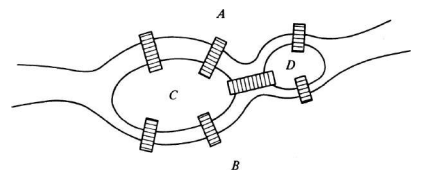
\includegraphics[width=0.3\textwidth]{./figures/bridge.png}
  \end{center}
  \caption{哥尼斯堡七桥问题现实模型}
\end{figure}

需要寻找方案(如果有的话)满足: 从某一块陆地出发,
经过每座桥且恰好经过一次并回到出发点.

欧拉通过用``点''表示陆地, 用``边''表示桥, 抽象出图的模型.
\begin{figure}[H]
  \begin{center}
    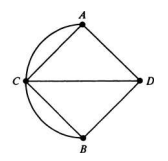
\includegraphics[width=0.2\textwidth]{./figures/bridge_graph.png}
  \end{center}
  \caption{哥尼斯堡七桥问题抽象模型}
\end{figure}

欧拉利用图的模型成功地证明了这个问题是不存在任何一种方案的.
但欧拉并不满足于此, 他还研究了什么样的图是存在这样的方案的(欧拉图),
这种做学问的精神是值得我们学习的, 关于欧拉图的进一步讨论可见有关的图论教材,
如\cite{ref5}, 这不在本文的讨论范围内.

\subsubsection{图的定义}
图(graph) $ G $ 定义为 $ G=(V, E) $, 其中 $ V $, $ E $ 是集合且
$ E \subseteq V\times V $. $ V $ 中的元素称作 $ G $ 的点(vertex), $ E $ 中的元素
称作 $ G $ 的边(edge). $ G $ 的点集记作 $ V(G) $, $ G $ 的边集记作 $ E(G) $.

对 $ x, y\in V(G) $, 边 $ \{x, y\} \in E(G) $记作$ xy $.
若 $ xy \in E(G) $, 则称点 $ x $ 和点 $ y $ 是相邻的(adjacent), 或称
点 $ x $ 和点 $ y $ 互为邻居(neighbors).

若图 $ G $ 的任意两点之间都是相邻的(pairwise adjacent), 则称 $ G $
是完全图(complete graph). 有 $ n $ 个点的完全图记作 $ K^{n} $, $ K^{3} $
称作三角形(triangle).

\subsection{名称解释}
\begin{itemize}
  \item 图: 图用于展示不同变量之间的关系,通常包括节点(点)和边(线)两部分。
    节点代表一个个体或对象,边则代表它们之间的关系。图可以用来解释复杂的关系网络和信息流动,
    如社交网络、交通网络、物流网络等。常见的图形类型包括有向图、无向图、树形图、地图等。
  \item Graph Processing:  Graph Processing是一种计算模型,用于处理图形数据结构的计算问题。
    图计算模型可以用于解决许多现实世界的问题,例如社交网络分析、网络流量分析、医疗诊断等,
    典型的系统有 Apache Giraph, Spark GraphX。
  \item DSL:  DSL是领域特定语言(Domain Specific Language)的缩写。
    它是一种针对特定领域或问题的编程语言,与通用编程语言不同,DSL主要关注于解决特定领域的问题,并针对该领域的特定需求进行优化。
    DSL可以使得编程更加简单、高效,同时也能够提高代码的可读性和可维护性。下面的Gremlin、ISO GQL就是DSL中的一种。
  \item HLA: HLA 是 High level language 的缩写,与DSL不同,它使用通用语言进行编程,Geaflow目前只支持Java程序编写。
    它主要通过计算引擎SDK进行程序编写,执行方式是将程序整体打包交给引擎执行,对比DSL,它的执行方式更加灵活,但相对应的编程也会更加复杂。
  \item Gremlin: Gremlin是一种图形遍历语言,用于在图形数据库中进行数据查询和操作。
    它是一种声明式的、基于图的编程语言,可以用于访问各种类型的图形数据库,如Apache TinkerPop、Neo4j等。
    它提供了一组灵活的API,可以帮助开发者在图形数据库中执行各种操作,如遍历、过滤、排序、连接、修改等。
  \item ISO GQL: GQL是面向属性图的标准查询语言,全称是“图形查询语言”,其为ISO/IEC国际标准数据库语言。
    GeaFlow不仅支持了Gremlin查询语言,而且还支持了GQL。
  \item Window: 参考VLDB 2015 Google Dataflow Model,窗口的概念在 Geaflow 中是其数据处理逻辑中的关键要素,用于统一有界和无界的数据处理。
    数据流统一被看成一个个窗口数据的集合,系统处理批次的粒度也就是窗口的粒度。
  \item Cycle: GeaFlow Scheduler调度模型中的核心数据结构,一个cycle描述为可循环执行的基本单元,包含输入,中间计算和数据交换,输出的描述。
    由执行计划中的vertex group生成,支持嵌套。
  \item Event: Runtime层调度和计算交互的核心数据结构,Scheduler将一系列Event集合构建成一个State Machine,将其分发到Worker上进行计算执行。
    其中有些Event是可执行的,即自身具备计算语义,整个调度和计算过程为异步执行。
  \item Graph Traversal: Graph Traversal 是指遍历图数据结构中所有节点或者部分节点的过程,在特定的顺序下访问所有节点,
    主要是深度优先搜索(DFS)和 广度优先搜索(BFS)。用于解决许多问题,包括查找两个节点之间的最短路径、检测图中的循环等。
  \item Graph State:  GraphState 是用来存放Geaflow的图数据或者图迭代计算过程的中间结果,提供Exactly Once语义,并提供作业级复用的能力。
    GraphState 分为 Static 和 Dynamic 两种,Static 的 GraphState 将整个图看做是一个完整的,
    所有操作都在一张全图上进行;Dynamic 的 GraphState 认为图动态变化的,由一个个时间切片构成,所有切片构成一个完整的图,
    所有的操作都是在切片上进行。
  \item Key State:  KeyState 用于存放计算过程中的中间结果,通常用于流式处理,例如执行aggregation时在KeyState中记录中间聚合结果。
    类似GraphState,Geaflow 会将 KeyState 定期持久化,因此KeyState也提供Exactly Once语义。
    KeyState根据数据结果不同可以分为KeyValueState、KeyListState、KeyMapState等。
\end{itemize}
